\documentclass[a4paper,12pt,numbered]{article}

\usepackage{mathtools}
\usepackage{amsmath}
\usepackage{soul}
\usepackage{amssymb,amsmath,amsfonts}
\usepackage[utf8]{inputenc}
\usepackage{graphicx}
\usepackage{geometry}
\usepackage{float}
\usepackage[german=quotes]{csquotes}
\usepackage{hyperref}
\usepackage{fancyhdr}
\usepackage{gensymb}
\usepackage{units}
\usepackage{hhline}
\usepackage{color}
\usepackage[export]{adjustbox}
\usepackage[nottoc,numbib]{tocbibind}
\usepackage[square,numbers]{natbib}
\usepackage{titling}
\usepackage{subfloat}
\usepackage{multicol}
\usepackage{caption}
\usepackage{authblk}
\usepackage{graphics}
\usepackage{subcaption}
\usepackage{pdfpages}

\begin{document}

\section{Neutrinos}



\section{A}

Neutrinos were first postulated by Wolfgang Pauli to explain the observed continous spectrum of the electron energy appearing during nuclear beta decay of Li-6 and nitrogen nuclei, as for a decay of a particle into two particles, the energy of the respective daughter particles can be calculated to be discrete values. Only for a decay into three or more particles can the energy spectrum of the electron in be continous. Thus Pauli postulated the existance of a third particle that does not interact electromagnetically without significant mass relative to the nucleus to explain the observations, the neutrino [cite pauli]. 
\\
Since then three different generations of neutrinos were discovered, the electron neutrino in 1956 at the Savannah River Plant, the muon neutrino in 1962 at the Brookhaven National Laboratory, and the tau neutrino in 2000 at Fermilab [cite review of neutrino history].

\subsection{B}

In the Standard Model (SM) each of these three generations of neutrinos are electromagnetically neutral, half-integer-spin particles that only interact through the weak force. The current composition of the SM is in Figure 1.


\begin{figure}[H]
\begin{center}
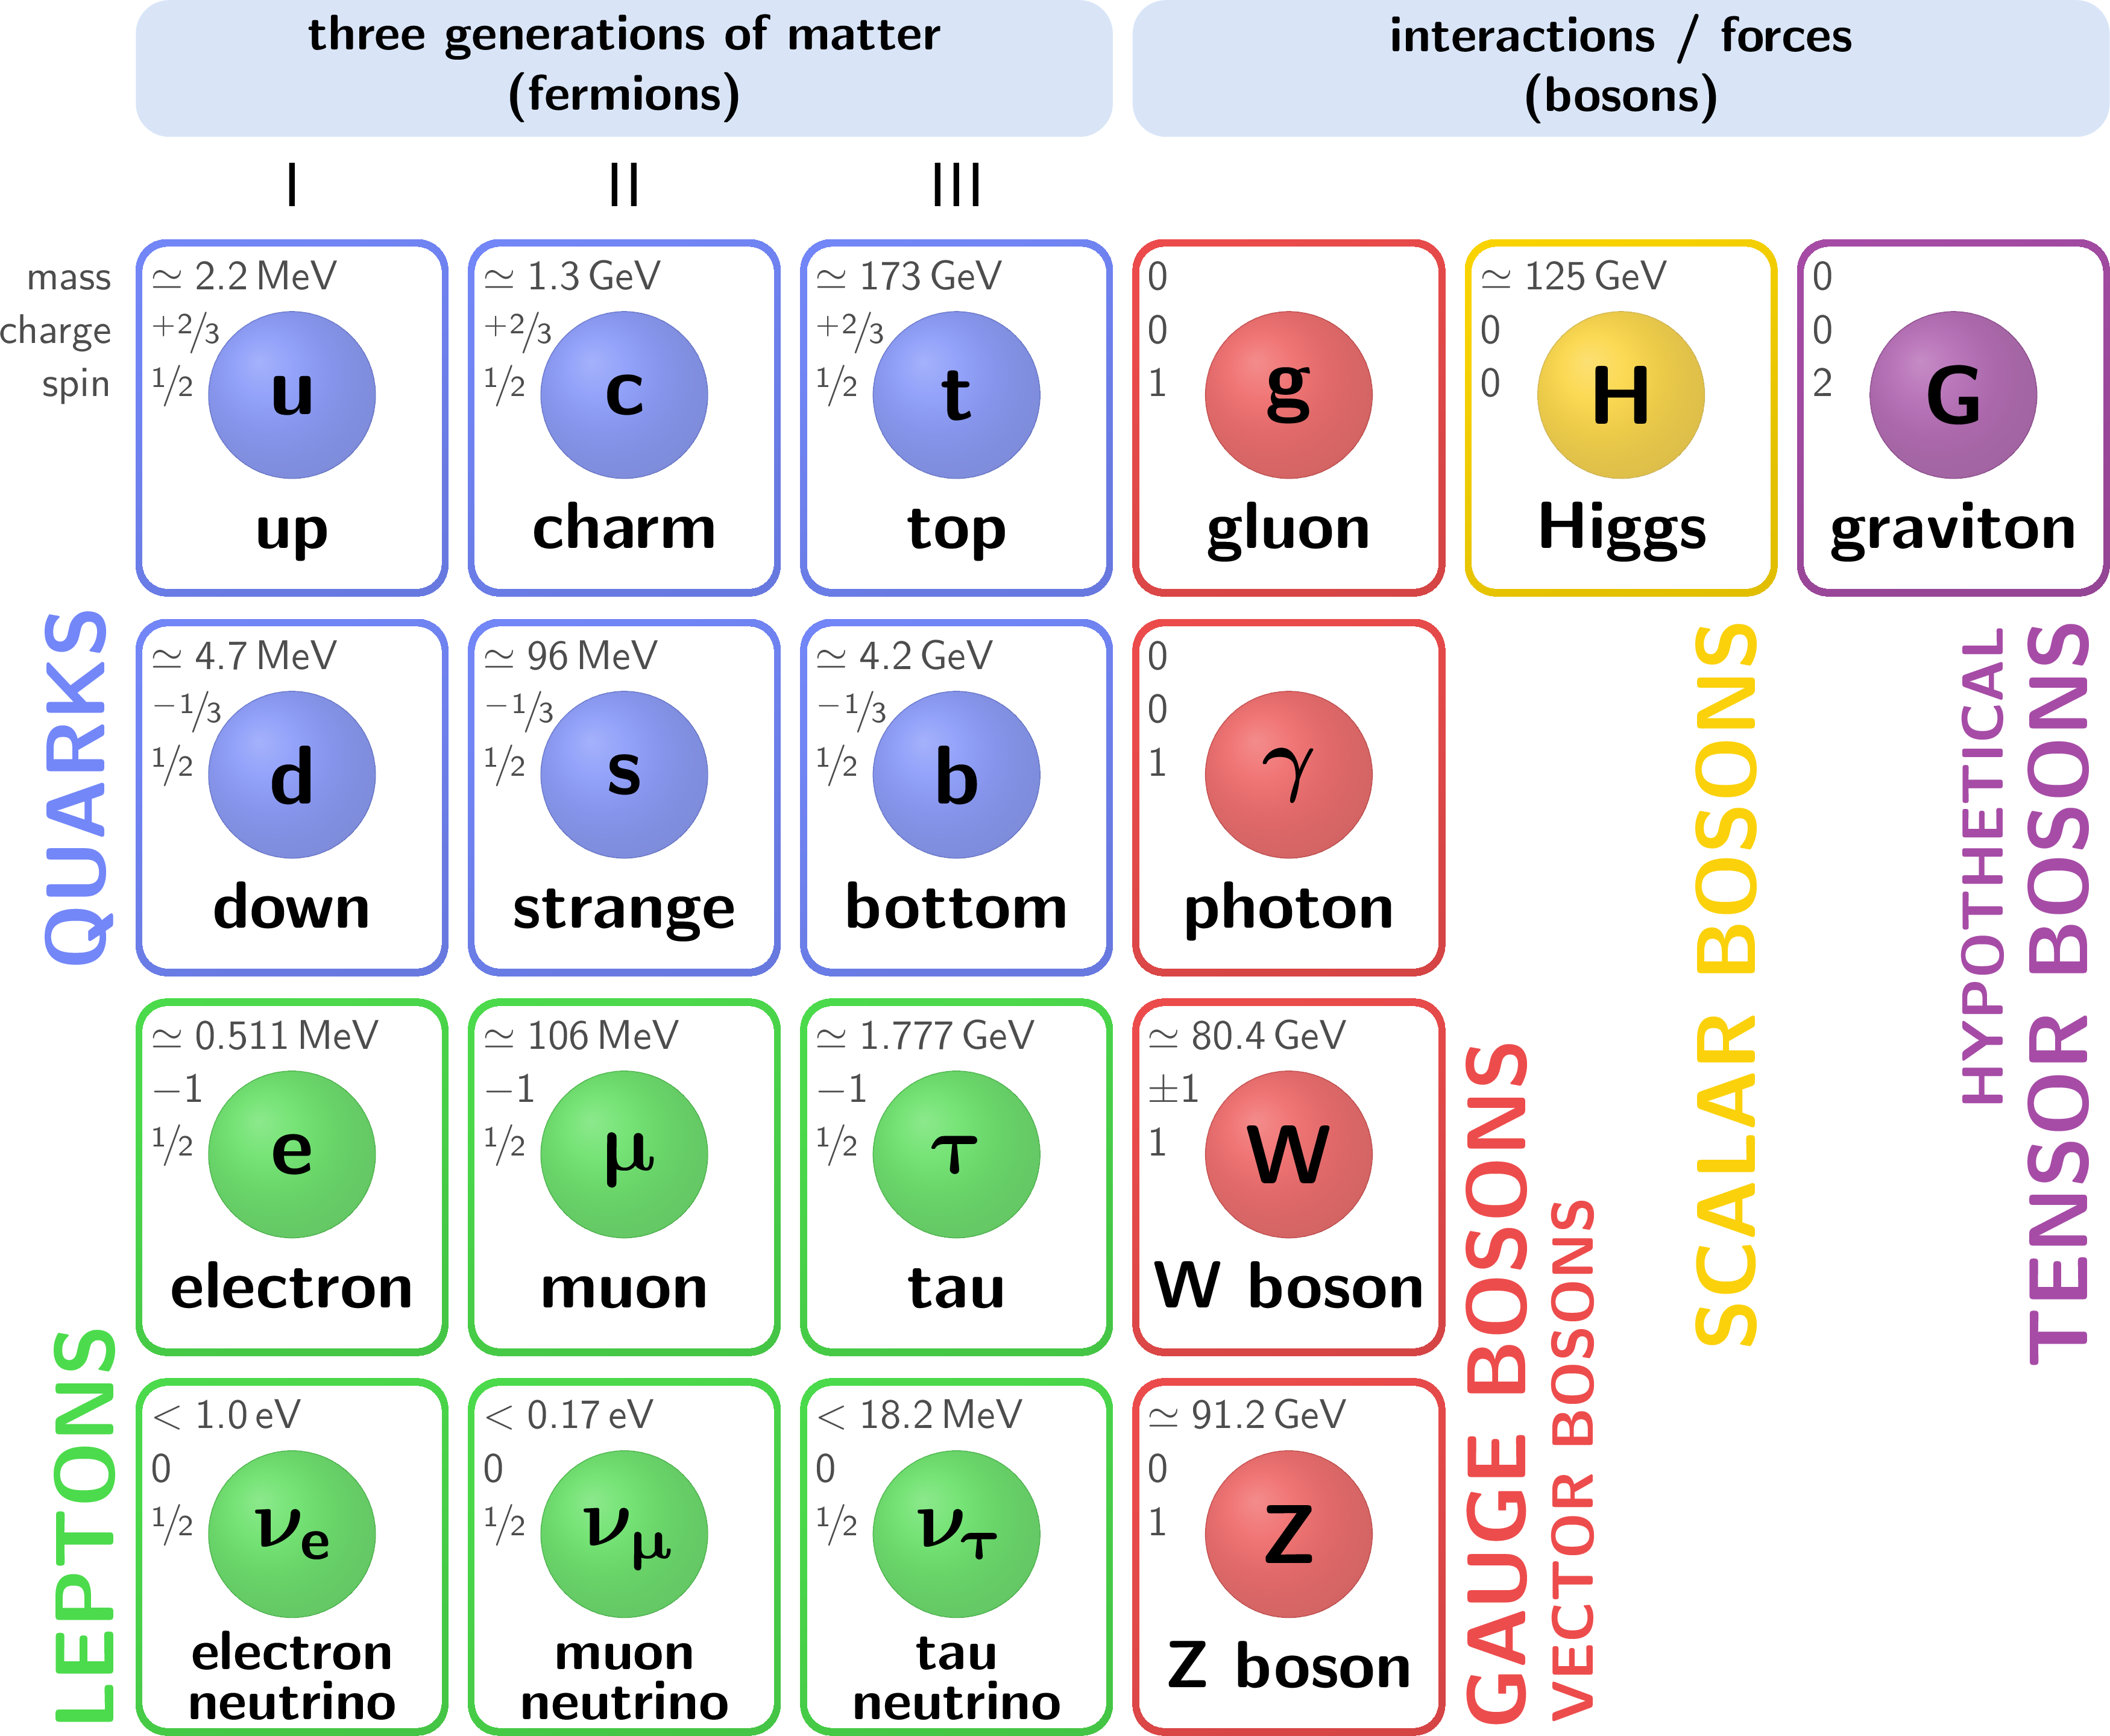
\includegraphics[width=0.80 \textwidth]{Neutrino_Figures/SM.png}
\caption{Standard Model, extracted from [cite]}
\end{center}
\end{figure}

Neutrinos have no mass in the SM as they are the only fermions in the SM that lack right-handed (left-handed in the case of antineutrinos) chiral counterparts and thus do not have a term in the SM Lagrangian to produce a Dirac mass $m \bar{u}_L u_R$, where $u_{R/L}$ are the right- and left-handed fermion fields respectively [maybe cite pdg review]. 
\\
Due to measurements of branching ratios the decay of Z-bosons, the number of active neutrinos $N_\nu$ is constrained to values of $N_\nu =3$ closely matching the number of existing generations of neutrinos [Cite Z-limits].

\subsection{C}

In 1998 Super-Kamiokande detector confirmed the oscillation of neutrino flavors by measuring the expected rate of muon neutrinos  with profound implications as oscillations of the neutrino flavors cannot happen with a non-zero mass [Cite superkamio]. Therefore it is clear that the SM needs to be extended.
The measured oscillations thus require the weak flavor eigenstates to each be made up of a mixing of the neutrino mass eigenstates due to the different phase speeds of each mass eigenstate caused by the different neutrino masses.

This mixing is codified in the unitary Pontecorvo-Maki-Nakagawa-Sakata (PMNS) matrix which describes the mixing from mass $\nu_{1/2/3}$ to flavor eigenstates $\nu_{e/\mu/\tau}$ with the mixing matrix elements labeled accordingly.

\begin{equation}
\begin{pmatrix}
\nu_e \\
\nu_\mu \\
\nu_\tau
\end{pmatrix}
=
\begin{pmatrix}
U_{e1} & U_{e2} & U_{e3} \\
U_{\mu 1} & U_{\mu 2} & U_{\mu 3} \\
U_{\tau 1} & U_{\tau 2} & U_{\tau 3}
\end{pmatrix}
\begin{pmatrix}
\nu_1 \\
\nu_2 \\
\nu_3
\end{pmatrix}
\end{equation}

This means that for a simplified two flavor model the oscillation probability can be described as follows

\begin{align}
\begin{split}
P(\nu_\alpha \rightarrow \nu_\beta) &= |\langle \nu_\beta(t) | \nu_\alpha(0) \rangle|^2 \\
&= \left| \sum_{i=1,2} U_{\beta i}^* U_{\alpha i} e^{-i E_i t} \right|^2 \\
&= \left| U_{\beta 1}^* U_{\alpha 1} + U_{\beta 2}^* U_{\alpha 2} e^{-i \frac{\Delta m^2 L}{2E}} \right|^2 \\
&= \sin^2(2\theta) \sin^2 \left( \frac{\Delta m^2 L}{4E} \right)
\end{split}
\end{align}

, where $\Theta$ corresponds to the angle of the rotation matrix between the two flavor and mass eigenstates. $\Delta m^2$ is the square of the mass difference (mass splitting) between the two mass states, $E$ the energy of the neutrino, and $L$ corresponds to the distance travelled by the neutrino.
\\
Neutrino experiments aimed at measuring the mass typically only produce restraints on the mass splitting and as such there remains the open question on the ordering of the neutrino masses [cite neutrino ordering review].

\begin{figure}[H]
\begin{center}
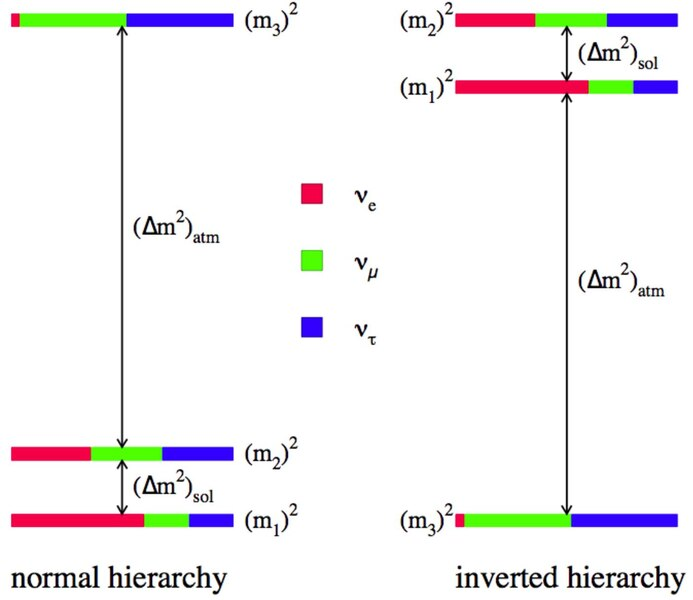
\includegraphics[width=0.75 \textwidth]{Neutrino_Figures/mass_ordering.jpg}
\caption{Neutrino mass ordering schemes and mass state composition, extracted from [cite]}
\end{center}
\end{figure}

For simplicity's sake this work will only consider normal ordering (NO) as shown in above figure. 

\subsection{D}

Due to neutrinos only interacting through the weak force, their interactions are limited to charged current (CC) and neutral current (NC) interactions with through the $W^{\pm}$ and Z Boson respectively.

leptons
Neutrino electon scattering
particle antiparticle scattering
nuclei
neutino quasi elastic scattering
neutral current elastic
resonant scattering
deep inelastic scattering

\subsubsection{E}

As neutrinos propagate through a medium they experience matter effects due to the presence of and interactions with electrons called the Mikheyev–Smirnov–Wolfenstein (MSW) effect [cite msw original paper]. In a two flavor approximation again, the addition of the mass potential from the electrons in a medium 

\begin{equation}
\mathcal{H}_\text{eff} = \frac{1}{2E} \begin{pmatrix} 
m_1^2 + 2 E V_\alpha & 0 \\
0 & m_2^2
\end{pmatrix}
\end{equation}

where $m_1^2$, $m_2^2$ are the mass eigenvalues of the neutrino states with NO, $E$ the energy of the neutrino, and $V_\alpha = \sqrt{2} G_F n_e$ the matter potential, where $G_F$ is the Fermi constant and $n_e$ is the electron number density in the medium.

The MSW effect can cause the conversion of one flavor to another when the effective mass squared difference is zero, which happens when $V_\alpha = \Delta m^2/2E$. The eigenvalues of the Hamiltonian desciribing the evolution of the neutrino states in equation (3) become the same at the resonance point allowing for conversion of flavors into one another.

\subsection{F}

\subsection{G}


\subsection{H}


The information about the following anomalies is taken from [cite sterile review].

\subsubsection{LSND}
\subsubsection{MiniBooNE}
\subsubsection{Reactor Anomaly}
\subsubsection{Gallium Anomaly}
\section{Sterile Neutrinos}

\subsection{I}

\bibliographystyle{unsrturl}

\bibliography{Bibtexquellen}

\end{document}


